

\documentclass[a4paper]{article}

\usepackage{amsmath}
\usepackage{hyperref}
\usepackage{biblatex}
\usepackage{enumerate}
\usepackage{graphicx}
\usepackage{stmaryrd}
\usepackage{listings}

\addbibresource{refs.bib}

\begin{document}

\author{Ola Bratt \\
  \href{mailto:ola.bratt@gmail.com}{ola.bratt@gmail.com}
}
\title{DAT565/DIT407 Assignment 1}
\date{2024-01-16}

\maketitle



\section*{Problem 1: Dependency Ratio}

In Figure~\ref{fig:ratio} the Dependecy Ratio of Sweden from 1860 to 2022 is show.
The ratio is calculated by using the data from SCB~\cite{SCB:2023}.



\begin{figure}[h]
  \begin{center}
    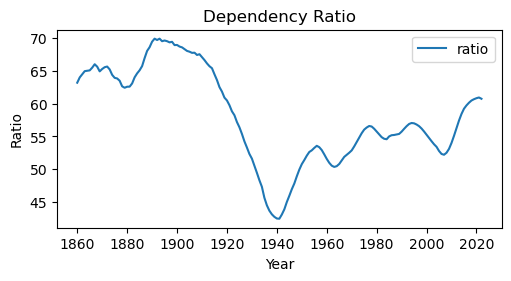
\includegraphics[width=\textwidth]{ratio.png}
    \caption{Dependecy ratio}
    \label{fig:ratio}
  \end{center}
\end{figure}

\newpage

In Figure~\ref{fig:fractions} the diffrent fractions of the population is shown. The fractions 
are calculated by dividing the population group (children, labor and elderly) with the total population. 
The fractions are calculated by using the data from SCB~\cite{SCB:2023}.


\begin{figure}[h]
  \begin{center}
    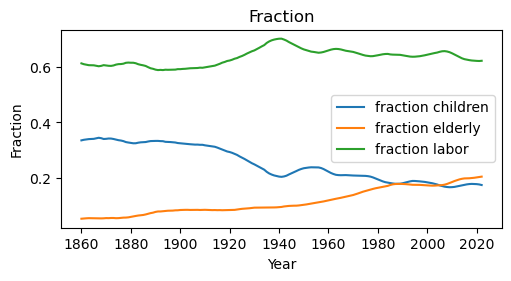
\includegraphics[width=\textwidth]{fractions.png}
    \caption{Fractions}
    \label{fig:fractions}
  \end{center}
\end{figure}


Discussion of results and general development of demographics trend of population
among industrialized countries.

Discuss the development of the Swedish population in light of these figures; how have the Swedish demographics changed over the years and why, and relate this to what you know (or can find out) about general trends of population among industrialized countries.



\printbibliography

\section*{Appendix: Source Code}
\lstinputlisting{assignment1.py}

\end{document}
